\documentclass[11pt, a4paper]{article}

% Fonts and Encoding
\usepackage[utf8]{inputenc}
\usepackage[T1]{fontenc}

% Math and Symbols
\usepackage{amsmath, amssymb, amsthm, amsfonts, mathrsfs, mathtools}

% Layout and Geometry
\usepackage{geometry}
\geometry{a4paper, margin=1in}

% Formatting and Graphics
\usepackage{graphicx, xcolor, enumitem, booktabs, array, tabularx}

% TikZ for Illustrations
\usepackage{tikz}
\usetikzlibrary{arrows.meta, positioning, shapes.geometric, calc, backgrounds, matrix}

% Clickable Links and TOC
\usepackage{hyperref}
\hypersetup{
    colorlinks=true,
    linkcolor=blue,
    filecolor=magenta,      
    urlcolor=cyan,
    pdftitle={Advanced Mathematics Topic},
}

% Theorem Environments
\newtheorem{theorem}{Theorem}[section]
\newtheorem{lemma}[theorem]{Lemma}
\newtheorem{proposition}[theorem]{Proposition}
\newtheorem{corollary}[theorem]{Corollary}
\theoremstyle{definition}
\newtheorem{definition}{Definition}[section]
\newtheorem{axiom}{Axiom}[section]
\newtheorem{example}{Example}[section]
\theoremstyle{remark}
\newtheorem{remark}{Remark}[section]

% Custom Commands (Enforced standard notation)
\newcommand{\R}{\mathbb{R}}
\newcommand{\N}{\mathbb{N}}
\newcommand{\Z}{\mathbb{Z}}
\newcommand{\Q}{\mathbb{Q}}
\newcommand{\E}{\mathbb{E}}
\newcommand{\Prob}{\mathbb{P}}
\newcommand{\F}{\mathcal{F}}

\begin{document}

\title{\textbf{Advanced Multivariate Probability Distributions: \\ The Expected Value of a Function of Random Variables}}
\author{Tashfeen Omran}
\date{\today}

\maketitle
\tableofcontents
\newpage

% ==========================================
% PART 1: Comprehensive Introduction
% ==========================================
\section{Comprehensive Introduction, Context, and Prerequisites}

\subsection{Core Concepts \& Axioms}
In the rigorous study of probability theory, we operate within a probability space $(\Omega, \F, \Prob)$, where $\Omega$ is the sample space, $\F$ is a $\sigma$-algebra of events, and $\Prob$ is a probability measure. A random variable $Y$ is a measurable function mapping $\Omega \to \R$. When we study complex, interacting systems, we must extend this to a \textit{random vector} $\mathbf{Y} = (Y_1, Y_2, \dots, Y_k)$, which maps $\Omega \to \R^k$.

The central focus of this document is determining the expected value of a scalar-valued function applied to a random vector, denoted as $g(Y_1, Y_2, \dots, Y_k)$. This is formally evaluated using the \textbf{Law of the Unconscious Statistician (LOTUS)}. LOTUS allows us to compute the expectation of $g(\mathbf{Y})$ directly from the joint probability distribution of $\mathbf{Y}$, without needing to derive the marginal distribution of the new random variable $Z = g(\mathbf{Y})$.

\subsection{Intuition and Measure-Theoretic Foundations}
Intuitively, the expected value is the center of mass of a distribution. When we apply a function $g$ to our random variables, we are warping the space $\R^k$ into a new space $\R$. Measure theory tells us that integrating the function $g(\mathbf{y})$ with respect to the pushforward measure induced by $\mathbf{Y}$ is equivalent to integrating $g(\mathbf{y})$ weighted by the joint density (or mass) function over the original space $\R^k$. 

If we partition the space $\R^k$ into infinitesimal hypercubes $d\mathbf{y}$, the probability mass in each hypercube is $f(\mathbf{y})d\mathbf{y}$. The expected value is simply the sum (or integral) of the function's value at each hypercube, weighted by this probability mass.

\subsection{Historical Context and Motivation}
The formalization of expected values for functions of multiple random variables was necessitated by the advent of statistical mechanics and early quantum theory in the late 19th and early 20th centuries. Physicists like Maxwell and Boltzmann needed to compute the expected kinetic energy of a gas, which is a function of the velocities of millions of interacting particles. Andrey Kolmogorov's 1933 axiomatization of probability using measure theory provided the rigorous bedrock that proved LOTUS was not just a heuristic, but a mathematically sound theorem derived from Lebesgue integration.

\subsection{Key Theorems, Lemmas, and Formulas}
\begin{theorem}[Multivariate LOTUS - Definition 5.9]
Let $g(Y_1, Y_2, \dots, Y_k)$ be a function of continuous random variables with joint probability density function $f(y_1, y_2, \dots, y_k)$. The expected value is given by:
\[
\E[g(Y_1, \dots, Y_k)] = \int_{-\infty}^{\infty} \cdots \int_{-\infty}^{\infty} g(y_1, \dots, y_k) f(y_1, \dots, y_k) \, dy_1 \dots dy_k
\]
For discrete random variables with joint probability mass function $p(y_1, \dots, y_k)$:
\[
\E[g(Y_1, \dots, Y_k)] = \sum_{y_1} \cdots \sum_{y_k} g(y_1, \dots, y_k) p(y_1, \dots, y_k)
\]
\end{theorem}

\begin{theorem}[Linearity of Expectation - Theorems 5.6 \& 5.7]
For any constants $c_1, c_2 \in \R$ and functions $g_1, g_2$:
\[
\E[c_1 g_1(Y_1, Y_2) + c_2 g_2(Y_1, Y_2)] = c_1 \E[g_1(Y_1, Y_2)] + c_2 \E[g_2(Y_1, Y_2)]
\]
\end{theorem}

\subsection{Prerequisites}
To master this topic, the reader must possess:
\begin{itemize}
    \item \textbf{Multivariable Calculus:} Proficiency in setting up and evaluating double and triple integrals, particularly over non-rectangular regions.
    \item \textbf{Foundational Probability:} Understanding of univariate density functions, cumulative distribution functions (CDFs), and independence.
    \item \textbf{Set Theory:} Ability to define regions of integration using set-builder notation and inequalities.
\end{itemize}

% ==========================================
% PART 2: Detailed Homework Solutions
% ==========================================
\section{Detailed Homework Solutions (Rigorous Proofs \& Computations)}

\subsection{Problem 5.68: The Bus and the Passenger}
\textbf{Problem Statement:} A bus arrives at a bus stop at a uniformly distributed time over the interval 0 to 1 hour. A passenger also arrives at a uniformly distributed time over the interval 0 to 1 hour. Assume arrival times are independent. The passenger will wait up to $1/4$ hour for the bus. What is the probability the passenger catches the bus?

\begin{proof}[Solution via Geometric Probability and Integration]
\textbf{Step 1: Define the Probability Space and Random Variables.}\\
Let $Y_1$ be the arrival time of the bus, and $Y_2$ be the arrival time of the passenger.
We are given that $Y_1 \sim U(0,1)$ and $Y_2 \sim U(0,1)$.
Because they are independent, the joint probability density function (PDF) is the product of their marginal PDFs:
\[
f(y_1, y_2) = f_{Y_1}(y_1) f_{Y_2}(y_2) = 1 \cdot 1 = 1, \quad \text{for} \quad 0 \leq y_1 \leq 1, \ 0 \leq y_2 \leq 1
\]
The joint density is 0 elsewhere.

\textbf{Step 2: Define the Event of Interest.}\\
The passenger catches the bus if and only if the bus arrives \textit{after} the passenger, but no more than $1/4$ hour after the passenger. Mathematically, this is the event $E$:
\[
E = \{ (y_1, y_2) \in \R^2 \mid y_2 \leq y_1 \leq y_2 + 1/4 \}
\]

\textbf{Step 3: Set up the Integral over the Region.}\\
We must integrate the joint PDF over the region $E$ bounded by the unit square $[0,1] \times [0,1]$.
The inequalities defining the region are:
1) $y_1 \geq y_2$ (The bus arrives after the passenger)
2) $y_1 \leq y_2 + 1/4 \implies y_2 \geq y_1 - 1/4$ (The passenger waits at most 1/4 hour)

We partition the integral with respect to $y_1$ into two intervals based on the intersection of the line $y_2 = y_1 - 1/4$ with the $y_1$-axis (which occurs at $y_1 = 1/4$):
For $0 \leq y_1 \leq 1/4$, the lower bound for $y_2$ is $0$.
For $1/4 \leq y_1 \leq 1$, the lower bound for $y_2$ is $y_1 - 1/4$.
The upper bound for $y_2$ is always $y_1$.

\textbf{Step 4: Evaluate the Integral.}\\
\begin{align*}
\Prob(E) &= \iint_E f(y_1, y_2) \, dy_2 \, dy_1 \\
&= \int_{0}^{1/4} \int_{0}^{y_1} 1 \, dy_2 \, dy_1 + \int_{1/4}^{1} \int_{y_1 - 1/4}^{y_1} 1 \, dy_2 \, dy_1 \\
&= \int_{0}^{1/4} [y_2]_{0}^{y_1} \, dy_1 + \int_{1/4}^{1} [y_2]_{y_1 - 1/4}^{y_1} \, dy_1 \\
&= \int_{0}^{1/4} y_1 \, dy_1 + \int_{1/4}^{1} \left( y_1 - \left(y_1 - \frac{1}{4}\right) \right) \, dy_1 \\
&= \left[ \frac{y_1^2}{2} \right]_{0}^{1/4} + \int_{1/4}^{1} \frac{1}{4} \, dy_1 \\
&= \frac{(1/4)^2}{2} + \frac{1}{4} \left( 1 - \frac{1}{4} \right) \\
&= \frac{1}{32} + \frac{1}{4} \left( \frac{3}{4} \right) = \frac{1}{32} + \frac{3}{16} = \frac{1}{32} + \frac{6}{32} = \frac{7}{32}
\end{align*}

\textbf{Conclusion:}\\
The probability that the passenger catches the bus is $\frac{7}{32}$.
\end{proof}

\subsection{Problem 5.69: Exponential Fuses}
\textbf{Problem Statement:} The length of life $Y$ for fuses is modeled by $f(y) = (1/3)e^{-y/3}$ for $y > 0$. 
(a) Find the joint PDF for two independent fuses $Y_1$ and $Y_2$. 
(b) Find $\Prob(Y_1 + Y_2 \leq 1)$.

\begin{proof}[Solution]
\textbf{Part (a): Joint Probability Density Function}\\
By the definition of independence, the joint PDF is the product of the marginal PDFs.
\begin{align*}
f(y_1, y_2) &= f_{Y_1}(y_1) f_{Y_2}(y_2) \\
&= \left( \frac{1}{3}e^{-y_1/3} \right) \left( \frac{1}{3}e^{-y_2/3} \right) \\
&= \frac{1}{9} e^{-(y_1 + y_2)/3}, \quad \text{for} \quad y_1 > 0, \ y_2 > 0
\end{align*}
The density is $0$ elsewhere.

\textbf{Part (b): Probability of Sum}\\
We seek $\Prob(Y_1 + Y_2 \leq 1)$. This requires integrating the joint PDF over the region where $y_1 + y_2 \leq 1$ in the first quadrant.
\begin{align*}
\Prob(Y_1 + Y_2 \leq 1) &= \int_{0}^{1} \int_{0}^{1 - y_1} \frac{1}{9} e^{-(y_1 + y_2)/3} \, dy_2 \, dy_1 \\
&= \int_{0}^{1} \frac{1}{3} e^{-y_1/3} \left( \int_{0}^{1 - y_1} \frac{1}{3} e^{-y_2/3} \, dy_2 \right) dy_1
\end{align*}
Evaluate the inner integral:
\begin{align*}
\int_{0}^{1 - y_1} \frac{1}{3} e^{-y_2/3} \, dy_2 &= \left[ -e^{-y_2/3} \right]_{0}^{1 - y_1} \\
&= -e^{-(1 - y_1)/3} - (-1) = 1 - e^{-(1 - y_1)/3}
\end{align*}
Substitute back into the outer integral:
\begin{align*}
\Prob(Y_1 + Y_2 \leq 1) &= \int_{0}^{1} \frac{1}{3} e^{-y_1/3} \left( 1 - e^{-(1 - y_1)/3} \right) dy_1 \\
&= \int_{0}^{1} \left( \frac{1}{3} e^{-y_1/3} - \frac{1}{3} e^{-y_1/3} e^{-1/3} e^{y_1/3} \right) dy_1 \\
&= \int_{0}^{1} \left( \frac{1}{3} e^{-y_1/3} - \frac{1}{3} e^{-1/3} \right) dy_1 \\
&= \left[ -e^{-y_1/3} - \frac{y_1}{3} e^{-1/3} \right]_{0}^{1} \\
&= \left( -e^{-1/3} - \frac{1}{3} e^{-1/3} \right) - \left( -e^{0} - 0 \right) \\
&= -\frac{4}{3} e^{-1/3} + 1 = 1 - \frac{4}{3} e^{-1/3}
\end{align*}

\textbf{Conclusion:}\\
The probability that the total effective life is less than or equal to 1 (hundred hours) is $1 - \frac{4}{3} e^{-1/3}$.
\end{proof}

\subsection{Problem 5.70: Supermarket Customers}
\textbf{Problem Statement:} $Y_1 \sim \text{Bin}(2, 0.2)$ and $Y_2 \sim \text{Bin}(1, 0.3)$ are independent. 
(a) Find the joint probability distribution. 
(b) Find the probability that not more than one customer spends over \$50 (i.e., $\Prob(Y_1 + Y_2 \leq 1)$).

\begin{proof}[Solution]
\textbf{Part (a): Joint Probability Distribution}\\
First, we compute the marginal probabilities for $Y_1$ and $Y_2$.
For $Y_1 \sim \text{Bin}(2, 0.2)$:
\begin{align*}
\Prob(Y_1 = 0) &= \binom{2}{0}(0.2)^0(0.8)^2 = 0.64 \\
\Prob(Y_1 = 1) &= \binom{2}{1}(0.2)^1(0.8)^1 = 0.32 \\
\Prob(Y_1 = 2) &= \binom{2}{2}(0.2)^2(0.8)^0 = 0.04
\end{align*}
For $Y_2 \sim \text{Bin}(1, 0.3)$:
\begin{align*}
\Prob(Y_2 = 0) &= \binom{1}{0}(0.3)^0(0.7)^1 = 0.7 \\
\Prob(Y_2 = 1) &= \binom{1}{1}(0.3)^1(0.7)^0 = 0.3
\end{align*}
Because $Y_1$ and $Y_2$ are independent, $p(y_1, y_2) = \Prob(Y_1 = y_1)\Prob(Y_2 = y_2)$. We construct the joint distribution table:

\vspace{10pt}
\renewcommand{\arraystretch}{1.5}
\noindent
\begin{tabularx}{\textwidth}{>{$\displaystyle}c<{$} >{$\displaystyle}X<{$} >{$\displaystyle}X<{$}}
\toprule
y_1 \setminus y_2 & 0 & 1 \\
\midrule
0 & (0.64)(0.7) = 0.448 & (0.64)(0.3) = 0.192 \\
1 & (0.32)(0.7) = 0.224 & (0.32)(0.3) = 0.096 \\
2 & (0.04)(0.7) = 0.028 & (0.04)(0.3) = 0.012 \\
\bottomrule
\end{tabularx}
\vspace{10pt}

\textbf{Part (b): Probability that $Y_1 + Y_2 \leq 1$}\\
We sum the probabilities of all disjoint events $(y_1, y_2)$ such that $y_1 + y_2 \leq 1$.
\begin{align*}
\Prob(Y_1 + Y_2 \leq 1) &= p(0,0) + p(1,0) + p(0,1) \\
&= 0.448 + 0.224 + 0.192 \\
&= 0.864
\end{align*}

\textbf{Conclusion:}\\
The probability that not more than one customer spends over \$50 is $0.864$.
\end{proof}

\subsection{Problem 5.71: Telephone Calls}
\textbf{Problem Statement:} Two calls arrive independently at random times in a 1-hour period. 
(a) Probability both are in the first half hour? 
(b) Probability they are within 5 minutes of each other?

\begin{proof}[Solution]
Let $Y_1, Y_2 \sim U(0, 60)$ minutes. The joint PDF is $f(y_1, y_2) = \frac{1}{60} \times \frac{1}{60} = \frac{1}{3600}$ for $0 \leq y_1, y_2 \leq 60$.

\textbf{Part (a): Both in the first half hour}\\
We seek $\Prob(Y_1 \leq 30 \cap Y_2 \leq 30)$. Due to independence:
\begin{align*}
\Prob(Y_1 \leq 30, Y_2 \leq 30) &= \Prob(Y_1 \leq 30) \Prob(Y_2 \leq 30) \\
&= \left( \frac{30}{60} \right) \left( \frac{30}{60} \right) = \frac{1}{2} \times \frac{1}{2} = \frac{1}{4}
\end{align*}

\textbf{Part (b): Within 5 minutes of each other}\\
We seek $\Prob(|Y_1 - Y_2| \leq 5)$. This is the area of the region $|y_1 - y_2| \leq 5$ inside the $60 \times 60$ square, multiplied by the uniform density $\frac{1}{3600}$.
The region is bounded by the lines $y_2 = y_1 + 5$ and $y_2 = y_1 - 5$.
Instead of integrating directly, we use geometric probability. The complement of this region consists of two identical right triangles in the corners of the square.
The upper-left triangle has vertices $(0,5), (0,60), (55,60)$. Its base and height are both $60 - 5 = 55$.
The lower-right triangle has vertices $(5,0), (60,0), (60,55)$. Its base and height are both $55$.
\begin{align*}
\text{Area of one triangle} &= \frac{1}{2} (55)(55) = \frac{3025}{2} \\
\text{Total area of complement} &= 2 \times \frac{3025}{2} = 3025 \\
\text{Area of desired region} &= 60^2 - 3025 = 3600 - 3025 = 575 \\
\Prob(|Y_1 - Y_2| \leq 5) &= \frac{575}{3600} = \frac{23}{144}
\end{align*}

\textbf{Conclusion:}\\
The probability the calls are within 5 minutes of each other is $\frac{23}{144}$.
\end{proof}

% ==========================================
% PART 3: In-Depth Analysis
% ==========================================
\section{In-Depth Analysis of Problems and Techniques}

\subsection{A) Problem Types and Logical Strategies}
\begin{itemize}
    \item \textbf{Geometric Probability (5.68, 5.71):} When dealing with independent uniform distributions, the joint density is constant. The strategy shifts from rigorous calculus to pure geometry. The probability is simply the ratio of the area of the target region to the area of the total sample space.
    \item \textbf{Convolution and Sums of Random Variables (5.69):} Finding the distribution of $Y_1 + Y_2$ requires integrating over a triangular region (a simplex). The overarching strategy is to fix one variable (e.g., $y_1$) and determine the dynamic bounds of the other ($0 \leq y_2 \leq 1 - y_1$).
    \item \textbf{Discrete Joint Distributions (5.70):} For discrete variables, integration is replaced by summation. The strategy is to construct an exhaustive matrix (table) of all possible state combinations, compute the joint probabilities via multiplication (due to independence), and sum the cells that satisfy the logical condition.
\end{itemize}

\subsection{B) Key Analytical and Logical Manipulations}
\begin{itemize}
    \item \textbf{Complementary Area Subtraction:} In Problem 5.71, integrating the absolute value inequality $|y_1 - y_2| \leq 5$ directly requires splitting the integral into multiple piecewise bounds. The logical trick is to calculate the area of the \textit{complement} (the two large triangles), which is mathematically trivial, and subtract it from the total area.
    \item \textbf{Dynamic Integration Bounds:} In Problem 5.68, the condition $y_2 \leq y_1 \leq y_2 + 1/4$ creates a slanted strip. The critical manipulation is recognizing that the lower bound of $y_2$ changes behavior at $y_1 = 1/4$, necessitating the splitting of the integral into $\int_0^{1/4}$ and $\int_{1/4}^1$.
\end{itemize}

% ==========================================
% PART 4: Cheatsheet, Visuals, and Tips
% ==========================================
\section{"Cheatsheet", Visuals, and Tips for Success}

\subsection{Visualizing Geometric Probability (Problem 5.68)}
The following TikZ diagram illustrates the integration region for the bus and passenger problem, demonstrating how inequalities map to geometric spaces.

\begin{center}
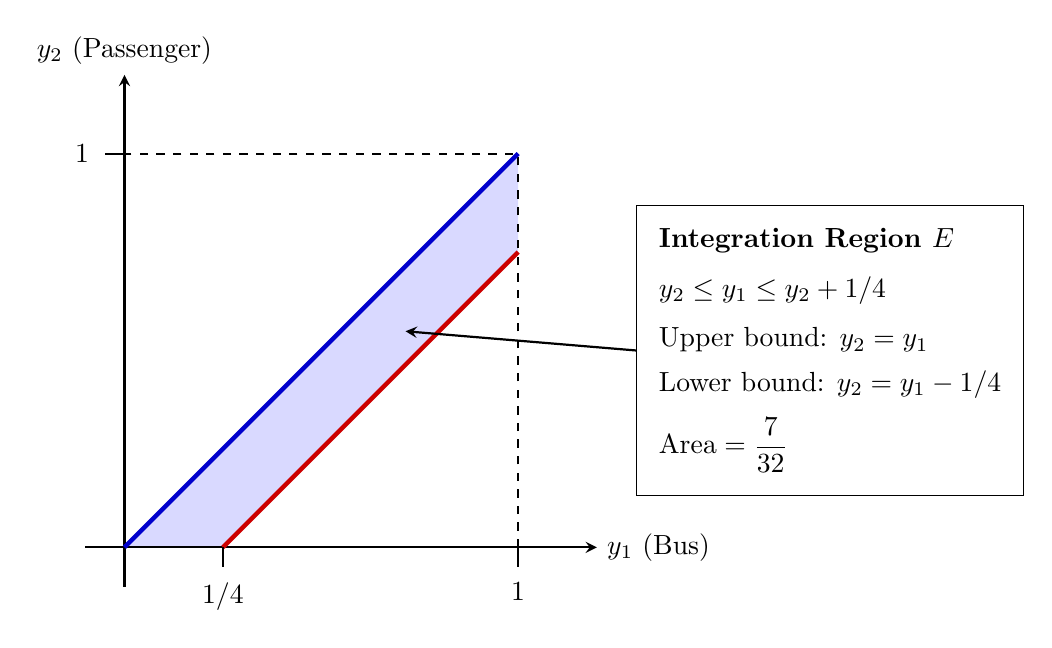
\begin{tikzpicture}[scale=5]
    % Background fill for the integration region
    \fill[blue!15] (0,0) -- (1,1) -- (1,0.75) -- (0.25,0) -- cycle;
    
    % Grid and axes
    \draw[thick, ->, >=stealth] (-0.1,0) -- (1.2,0) node[right] {$y_1$ (Bus)};
    \draw[thick, ->, >=stealth] (0,-0.1) -- (0,1.2) node[above] {$y_2$ (Passenger)};
    \draw[dashed, thick] (1,0) -- (1,1) -- (0,1);
    
    % Primary plots (Lines)
    \draw[ultra thick, blue!80!black] (0,0) -- (1,1);
    \draw[ultra thick, red!80!black] (0.25,0) -- (1,0.75);
    
    % Tick marks and labels
    \draw[thick] (1,0) -- (1,-0.05) node[below=2pt] {$\displaystyle 1$};
    \draw[thick] (0.25,0) -- (0.25,-0.05) node[below=2pt] {$\displaystyle 1/4$};
    \draw[thick] (0,1) -- (-0.05,1) node[left=2pt] {$\displaystyle 1$};
    
    % Single-Node Multiline Legend
    \node[align=left, anchor=west, inner sep=8pt, draw, fill=white] at (1.3, 0.5) {
        \textbf{Integration Region $E$} \\[6pt]
        $\displaystyle y_2 \leq y_1 \leq y_2 + 1/4$ \\[6pt]
        Upper bound: $y_2 = y_1$ \\[4pt]
        Lower bound: $y_2 = y_1 - 1/4$ \\[6pt]
        $\displaystyle \text{Area} = \frac{7}{32}$
    };
    
    % Callout arrow
    \draw[->, >=stealth, shorten >=2pt, thick] (1.3, 0.5) -- (0.7, 0.55);
\end{tikzpicture}
\end{center}

\subsection{Heuristics \& "Cheats"}
\begin{itemize}
    \item \textbf{The Independence Shortcut:} If $Y_1, Y_2$ are independent, and the region of integration is rectangular (e.g., $a \leq Y_1 \leq b$ and $c \leq Y_2 \leq d$), the double integral perfectly factors into the product of two single integrals.
    \item \textbf{The Absolute Value Trick:} Inequalities of the form $|X - Y| \leq c$ always form a diagonal strip through the origin. Always use the complementary triangle area method to solve these.
\end{itemize}

\subsection{Pitfalls \& Fallacies}
\begin{itemize}
    \item \textbf{The Non-Linear Expectation Fallacy:} Assuming $\E[g(Y_1, Y_2)] = g(\E[Y_1], \E[Y_2])$. This is strictly false unless $g$ is a linear function. For example, $\E[Y_1 Y_2] \neq \E[Y_1]\E[Y_2]$ if the variables are correlated.
    \item \textbf{Static Bounds Trap:} When integrating over a region like $Y_1 + Y_2 \leq 1$, a common fatal error is setting the bounds as $\int_0^1 \int_0^1 \dots dy_2 dy_1$. The inner bound \textit{must} be a function of the outer variable (e.g., $1 - y_1$).
\end{itemize}

% ==========================================
% PART 5: Conceptual Synthesis
% ==========================================
\section{Conceptual Synthesis and The "Big Picture"}

\subsection{A) Thematic Connections}
The central theme of this chapter is \textbf{measure-theoretic aggregation}. We are learning how to take a multi-dimensional probability space (the joint distribution) and collapse it down to a single scalar value (the expectation) via a transformation function $g$. This unifies previous topics: the univariate expected value is simply a special case where the mapping is from $\R^1 \to \R$, and marginalization is a special case where $g(Y_1, Y_2) = Y_1$.

\subsection{B) Forward and Backward Links}
\begin{itemize}
    \item \textbf{Backward Links:} This builds directly on multivariable calculus (Fubini's Theorem for swapping integral bounds) and basic set theory (defining intersections of events).
    \item \textbf{Forward Links:} Understanding how to integrate functions of multiple random variables is the absolute bedrock for \textbf{Covariance and Correlation} (where $g(Y_1, Y_2) = (Y_1 - \mu_1)(Y_2 - \mu_2)$). Furthermore, it is the foundation for \textbf{Stochastic Calculus}, where we must evaluate the expected payoff of financial derivatives that depend on multiple underlying stochastic assets.
\end{itemize}

% ==========================================
% PART 6: Abstract Real-World Modeling
% ==========================================
\section{Abstract Real-World Modeling (AI, ML, \& Quant Finance)}

\subsection{A) Concrete Scenarios}
\begin{enumerate}
    \item \textbf{Quantitative Finance (Basket Options):} A basket option's payoff depends on the weighted sum of multiple underlying assets. Pricing this derivative requires computing the expected value of a non-linear function $g(S_1, S_2) = \max(w_1 S_1 + w_2 S_2 - K, 0)$ under a risk-neutral probability measure.
    \item \textbf{Machine Learning (Loss Functions):} In Bayesian Neural Networks, weights are treated as random variables $\mathbf{W}$. The expected generalization error is the expected value of the loss function $L(\mathbf{W}, \mathbf{X}, \mathbf{y})$ integrated over the joint posterior distribution of the weights.
\end{enumerate}

\subsection{B) Model Problem Setup: Pricing a Spread Option}
Let us build a rigorous mathematical model for a Quant Finance scenario. We wish to price a European spread option, which pays out based on the difference between two asset prices at maturity $T$.

\textbf{State Space \& Random Variables:}
Let $(\Omega, \F, \mathbb{Q})$ be a risk-neutral probability space. Let $S_1(T)$ and $S_2(T)$ be the prices of two assets at time $T$. Assume they follow a bivariate log-normal distribution such that $Y_1 = \ln S_1(T)$ and $Y_2 = \ln S_2(T)$ are jointly normal with means $\mu_1, \mu_2$, variances $\sigma_1^2, \sigma_2^2$, and correlation $\rho$.

\textbf{The Function $g$:}
The payoff function of the spread option with strike $K$ is:
\[
g(S_1, S_2) = \max(S_1 - S_2 - K, 0)
\]

\textbf{The Optimization/Pricing Problem:}
By the Fundamental Theorem of Asset Pricing, the fair price $V_0$ of the option is the discounted expected value of the payoff under the risk-neutral measure $\mathbb{Q}$:
\[
V_0 = e^{-rT} \E^{\mathbb{Q}}[g(S_1(T), S_2(T))]
\]
Using LOTUS, this requires evaluating the following integral over $\R^2$:
\[
V_0 = e^{-rT} \iint_{\R^2} \max(e^{y_1} - e^{y_2} - K, 0) f_{Y_1, Y_2}(y_1, y_2) \, dy_1 \, dy_2
\]
where $f_{Y_1, Y_2}$ is the bivariate normal density. Because the $\max$ function introduces a non-linear kink, this integral generally lacks a closed-form solution and requires numerical integration or Margrabe's Formula (if $K=0$). This demonstrates how LOTUS is directly applied in algorithmic trading and derivatives pricing.

% ==========================================
% PART 7: Common Variations
% ==========================================
\section{Common Variations and Untested Concepts}

A critical concept not covered in the provided homework is the \textbf{Expected Value of a Product of Correlated Variables}. The homework only tested independent variables.

\begin{theorem}[Expectation of a Product]
If $Y_1$ and $Y_2$ are \textit{not} independent, $\E[Y_1 Y_2] = \E[Y_1]\E[Y_2] + \text{Cov}(Y_1, Y_2)$.
\end{theorem}

\textbf{Worked Example:}
Let $Y_1, Y_2$ have joint density $f(y_1, y_2) = y_1 + y_2$ for $0 \leq y_1 \leq 1, 0 \leq y_2 \leq 1$. Find $\E[Y_1 Y_2]$.
\begin{proof}
\begin{align*}
\E[Y_1 Y_2] &= \int_{0}^{1} \int_{0}^{1} y_1 y_2 (y_1 + y_2) \, dy_1 \, dy_2 \\
&= \int_{0}^{1} \int_{0}^{1} (y_1^2 y_2 + y_1 y_2^2) \, dy_1 \, dy_2 \\
&= \int_{0}^{1} \left[ \frac{y_1^3}{3} y_2 + \frac{y_1^2}{2} y_2^2 \right]_{0}^{1} dy_2 \\
&= \int_{0}^{1} \left( \frac{1}{3} y_2 + \frac{1}{2} y_2^2 \right) dy_2 \\
&= \left[ \frac{y_2^2}{6} + \frac{y_2^3}{6} \right]_{0}^{1} = \frac{1}{6} + \frac{1}{6} = \frac{1}{3}
\end{align*}
\end{proof}

% ==========================================
% PART 8: Advanced Diagnostic Testing
% ==========================================
\section{Advanced Diagnostic Testing: "Find the Flaw"}

Below are five proofs containing a single, subtle logical or mathematical flaw. 

\textbf{Problem 1:} Let $Y_1, Y_2 \sim U(0,1)$ be independent. We wish to find $\E[Y_1 / Y_2]$.
\textit{Flawed Proof:} By linearity of expectation and independence, $\E[Y_1 / Y_2] = \E[Y_1] / \E[Y_2]$. Since $\E[Y_1] = 0.5$ and $\E[Y_2] = 0.5$, the expected value is $0.5 / 0.5 = 1$.

\textbf{Problem 2:} Let $Y_1, Y_2$ be random variables such that $\E[Y_1 Y_2] = \E[Y_1]\E[Y_2]$.
\textit{Flawed Proof:} Because the expectation of the product equals the product of the expectations, $Y_1$ and $Y_2$ are independent random variables.

\textbf{Problem 3:} Let $f(y_1, y_2) = 2$ for $0 \leq y_2 \leq y_1 \leq 1$. Find the marginal density $f_{Y_1}(y_1)$.
\textit{Flawed Proof:} To find the marginal density of $Y_1$, we integrate out $y_2$ over its entire support from $0$ to $1$. $f_{Y_1}(y_1) = \int_0^1 2 \, dy_2 = 2[y_2]_0^1 = 2$.

\textbf{Problem 4:} Let $Y_1, Y_2 \sim U(0,1)$ be independent. Find the distribution of $Z = Y_1 + Y_2$.
\textit{Flawed Proof:} Since $Y_1$ ranges from 0 to 1, and $Y_2$ ranges from 0 to 1, their sum $Z$ must range from 0 to 2. Because both are uniformly distributed, their sum is also uniformly distributed. Thus, $Z \sim U(0,2)$.

\textbf{Problem 5:} Let $Y_1, Y_2$ have joint density $f(y_1, y_2) = e^{-y_1 - y_2}$ for $y_1, y_2 > 0$. Find $\E[e^{Y_1 + Y_2}]$.
\textit{Flawed Proof:} Using LOTUS, $\E[e^{Y_1 + Y_2}] = \int_0^\infty \int_0^\infty e^{y_1 + y_2} e^{-y_1 - y_2} \, dy_1 \, dy_2 = \int_0^\infty \int_0^\infty 1 \, dy_1 \, dy_2 = \infty$.

\vspace{10pt}
\hrule
\vspace{10pt}

\subsection*{Solution Key: Resolutions to the Flaws}
\begin{itemize}
    \item \textbf{Resolution 1:} The flaw is assuming $\E[1/Y_2] = 1/\E[Y_2]$. By Jensen's Inequality, since $g(x) = 1/x$ is strictly convex for $x>0$, $\E[1/Y_2] > 1/\E[Y_2]$. In fact, $\int_0^1 (1/y_2) dy_2$ diverges to infinity.
    \item \textbf{Resolution 2:} The flaw is affirming the consequent. $\E[Y_1 Y_2] = \E[Y_1]\E[Y_2]$ only implies that the variables are \textit{uncorrelated} (covariance is zero). Uncorrelated does not imply independent (unless the variables are jointly normal).
    \item \textbf{Resolution 3:} The flaw is using static bounds for $y_2$. The support of $y_2$ is bounded by $y_1$. The correct integral is $f_{Y_1}(y_1) = \int_0^{y_1} 2 \, dy_2 = 2y_1$.
    \item \textbf{Resolution 4:} The flaw is assuming the sum of uniforms is uniform. The convolution of two uniform distributions yields a triangular distribution (the Irwin-Hall distribution), not a uniform one.
    \item \textbf{Resolution 5:} The math is actually correct, but the logical flaw is failing to state that the expected value \textit{does not exist} (or diverges). An expectation is only formally defined if the integral of the absolute value is finite.
\end{itemize}

\end{document}